% Seminarul 16: Recapitulare
% Statistica piețelor financiare -- Program de licență, Academia de Studii Economice din București
% GENERAT de latex/build_seminar16.py -- modificați generatorul, nu acest fișier.
% Implicit versiunea pentru studenți; versiunea profesorului este wrapper-ul *_solutions.tex.
\makeatletter\@ifundefined{ifsolutions}{\expandafter\newif\csname ifsolutions\endcsname}{}\makeatother

\newcommand{\coursename}{Statistica piețelor financiare}
\def\sfmlang{ro}
% Preambul comun SFM -- Statistica piețelor financiare / Statistics of Financial Markets (Beamer, 16:9)
% Același design ca MFM. Înainte de % Preambul comun SFM -- Statistica piețelor financiare / Statistics of Financial Markets (Beamer, 16:9)
% Același design ca MFM. Înainte de % Preambul comun SFM -- Statistica piețelor financiare / Statistics of Financial Markets (Beamer, 16:9)
% Același design ca MFM. Înainte de \input{../../latex/preamble} se definește
%   \newcommand{\coursename}{Statistics of Financial Markets}      (EN)
%   \newcommand{\coursename}{Statistica piețelor financiare}       (RO)  și  \def\sfmlang{ro}
% Fișierele .tex se află în EN/Courses, EN/Seminars, RO/Cursuri, RO/Seminarii (două niveluri sub rădăcină).
% Deck-urile sînt generate de latex/build_chapterN.py / build_seminarN.py (vezi latex/sfm_build.py).

\documentclass[9pt, aspectratio=169, t]{beamer}
\providecommand{\coursename}{Statistics of Financial Markets}

% Ensure content fits on slides
\setbeamersize{text margin left=8mm, text margin right=8mm}

%=============================================================================
% THEME AND STYLE CONFIGURATION
%=============================================================================
\usetheme{default}
% Using default theme for clean header/footer control

% Color Palette (matching Redispatch PDF)
\definecolor{MainBlue}{RGB}{26, 58, 110}
\definecolor{AccentBlue}{RGB}{26, 58, 110}
\definecolor{IDAred}{RGB}{205, 0, 0}
\definecolor{DarkGray}{RGB}{51, 51, 51}
\definecolor{MediumGray}{RGB}{128, 128, 128}
\definecolor{LightGray}{RGB}{248, 248, 248}
\definecolor{VeryLightGray}{RGB}{235, 235, 235}
\definecolor{KeynoteGray}{RGB}{218, 218, 218}
\definecolor{SectionGray}{RGB}{120, 120, 120}
\definecolor{FooterGray}{RGB}{100, 100, 100}
\definecolor{Crimson}{RGB}{220, 53, 69}
\definecolor{Forest}{RGB}{46, 125, 50}
\definecolor{Amber}{RGB}{181, 133, 63}
\definecolor{Orange}{RGB}{230, 126, 34}
\definecolor{Purple}{RGB}{142, 68, 173}

% Gradient background (exact Keynote 315° gradient: white to RGB 218,218,218)
\setbeamertemplate{background}{%
    \begin{tikzpicture}[remember picture, overlay]
        \shade[shading=axis, shading angle=315,
        top color=white, bottom color=KeynoteGray]
        (current page.south west) rectangle (current page.north east);
    \end{tikzpicture}%
}
% Fallback solid color for compatibility
\setbeamercolor{background canvas}{bg=}

\setbeamercolor{palette primary}{bg=MainBlue, fg=white}
\setbeamercolor{palette secondary}{bg=MainBlue!85, fg=white}
\setbeamercolor{palette tertiary}{bg=MainBlue!70, fg=white}
\setbeamercolor{structure}{fg=MainBlue}
\setbeamercolor{title}{fg=IDAred}
\setbeamercolor{frametitle}{fg=IDAred, bg=}
\setbeamercolor{block title}{bg=MainBlue, fg=white}
\setbeamercolor{block body}{bg=VeryLightGray, fg=DarkGray}
\setbeamercolor{block title alerted}{bg=Crimson, fg=white}
\setbeamercolor{block body alerted}{bg=Crimson!8, fg=DarkGray}
\setbeamercolor{block title example}{bg=Forest, fg=white}
\setbeamercolor{block body example}{bg=Forest!8, fg=DarkGray}
\setbeamercolor{item}{fg=MainBlue}

% Footer colors (override Madrid theme blue)
\setbeamercolor{author in head/foot}{fg=FooterGray, bg=}
\setbeamercolor{title in head/foot}{fg=FooterGray, bg=}
\setbeamercolor{date in head/foot}{fg=FooterGray, bg=}
\setbeamercolor{section in head/foot}{fg=FooterGray, bg=}
\setbeamercolor{subsection in head/foot}{fg=FooterGray, bg=}

% Bullet styles (apply everywhere including blocks)
\setbeamertemplate{itemize item}{\color{MainBlue}$\boxdot$}
\setbeamertemplate{itemize subitem}{\color{MainBlue}$\blacktriangleright$}
\setbeamertemplate{itemize subsubitem}{\color{MainBlue}\tiny$\bullet$}
\setbeamertemplate{itemize/enumerate body begin}{\normalsize}
\setbeamertemplate{itemize/enumerate subbody begin}{\normalsize}

% Item spacing - compact style
\setlength{\leftmargini}{10pt}       % Level 1: minimal indent
\setlength{\leftmarginii}{10pt}      % Level 2: minimal additional indent
% Compact list spacing (zero extra space before/after lists in blocks)
\makeatletter
\def\@listi{\leftmargin\leftmargini \topsep 0pt \parsep 0pt \itemsep 0pt}
\def\@listii{\leftmargin\leftmarginii \topsep 0pt \parsep 0pt \itemsep 0pt}
\makeatother

\setbeamertemplate{navigation symbols}{}

%=============================================================================
% CUSTOM HEADLINE
%=============================================================================
\setbeamertemplate{headline}{%
    \vskip10pt%
    \hbox to \paperwidth{%
        \hskip0.5cm%
        {\small\color{FooterGray}\renewcommand{\hyperlink}[2]{##2}\insertsectionhead}%
        \hfill%
        \textcolor{FooterGray}{\small\insertframenumber}%
        \hskip0.5cm%
    }%
    \vskip4pt%
    {\color{FooterGray}\hrule height 0.4pt}%
}

%=============================================================================
% CUSTOM FOOTER
%=============================================================================
\usepackage{fontawesome5}

\setbeamertemplate{footline}{%
    {\color{FooterGray}\hrule height 0.4pt}%
    \vskip4pt%
    \hbox to \paperwidth{%
        \hskip0.5cm%
        \textcolor{FooterGray}{\small\coursename}%
        \hfill%
        \raisebox{-0.1em}{%
            \begin{tikzpicture}[x=0.08em, y=0.08em, line width=0.4pt]
                \draw[FooterGray] (0,3) -- (1,4) -- (2,3.5) -- (3,5) -- (4,4) -- (5,6) -- (6,5.5) -- (7,4) -- (8,5) -- (9,7) -- (10,6) -- (11,5) -- (12,6.5) -- (13,8) -- (14,7) -- (15,6) -- (16,7.5) -- (17,9) -- (18,8) -- (19,7) -- (20,8.5) -- (21,10) -- (22,9) -- (23,8) -- (24,9.5);
            \end{tikzpicture}%
        }%
        \hskip0.5cm%
    }%
    \vskip6pt%
}

%=============================================================================
% PACKAGES
%=============================================================================
\usepackage[utf8]{inputenc}
\DeclareUnicodeCharacter{03B1}{\ensuremath{\alpha}}
\usepackage[T1]{fontenc}
\usepackage{amsmath, amssymb, amsthm}
\usepackage{mathtools}
\usepackage{bm}
\usepackage{tikz}
\usetikzlibrary{arrows.meta, positioning, shapes, calc, decorations.pathreplacing, shadings}
\usepackage{booktabs}
\usepackage{multirow}
\usepackage{array}
\usepackage{graphicx}
\usepackage{hyperref}
\usepackage{colortbl}
\usepackage{listings}
\lstset{language=Python, basicstyle=\ttfamily\scriptsize, keywordstyle=\color{MainBlue}\bfseries,
  commentstyle=\color{Forest}, stringstyle=\color{Crimson}, breaklines=true,
  frame=none, backgroundcolor=\color{VeryLightGray}, xleftmargin=2mm}
\hypersetup{colorlinks=true, linkcolor=MainBlue, urlcolor=MainBlue}
\graphicspath{{../../logos/}{../../charts/}{../../photos/}}
\usepackage{xcolor}
\hfuzz=2pt  % Suppress tiny overfull warnings (<2pt)
\vfuzz=2pt  % Suppress tiny vertical overfull warnings (<2pt)

%=============================================================================
% QUANTLET COMMANDS
%   \quantlet{<displayed name>}{<url>}       (generic, compatible with the older SFM decks)
%   \sfmquantlet{Ch_05}{SFM_ch5_garch}       -> https://github.com/danpele/SFM/tree/main/Quantlets/Ch_05/SFM_ch5_garch
%   \qlurl{<folder>} is defined per chapter by the generator (Quantlets/Ch_NN/<folder>)
%=============================================================================
\newcommand{\sfmrepo}{https://github.com/danpele/SFM}
\newcommand{\sfmqlbase}{https://github.com/danpele/SFM/tree/main/Quantlets}
\newcommand{\quantlet}[2]{%
    \hfill\href{#2}{%
        \raisebox{-0.15em}{
\includegraphics[height=0.7em]{ql_logo.png}}%
        \textcolor{MainBlue}{\tiny\ #1}%
    }%
}
\newcommand{\sfmquantlet}[2]{\quantlet{\detokenize{#2}}{\sfmqlbase/#1/#2}}

%=============================================================================
% NOTEBOOKS (Google Colab)
%   \colaburl{notebooks/EN/chapter5_seminar_notebook.ipynb} -> the Colab link of a file in the SFM repo
%   \nb: the chapter notebook (each seminar deck redefines it with \renewcommand)
%=============================================================================
\newcommand{\colaburl}[1]{https://colab.research.google.com/github/danpele/SFM/blob/main/#1}
\newcommand{\nb}{https://colab.research.google.com/github/danpele/SFM/tree/main/notebooks/EN}
\newcommand{\nbname}{notebooks/EN}

%=============================================================================
% SLIDE HELPERS (used by the generators; the same as in MFM)
%=============================================================================
% local font size for list bodies (the preamble forces \normalsize)
\newcommand{\itemsize}[1]{\setbeamertemplate{itemize/enumerate body begin}{#1}\setbeamertemplate{itemize/enumerate subbody begin}{#1}}
\newcommand{\intitle}[1]{{\hypersetup{urlcolor=white}#1}}   % white links inside coloured title bars
\newcommand{\imgcap}[1]{{\scriptsize #1}\\[0.5mm]}          % caption under a photo
\newcommand{\imgcredit}[2]{{\tiny\color{FooterGray}\href{#1}{#2}}}   % image credit: source URL, author/licence
\newcommand{\aiprompt}[1]{{\ttfamily\color{MainBlue}#1}}     % a prompt to an AI assistant

%=============================================================================
% SEMINARS: student version by default; the instructor wrapper *_solutions.tex sets \solutionstrue
%=============================================================================
\makeatletter\@ifundefined{ifsolutions}{\expandafter\newif\csname ifsolutions\endcsname}{}\makeatother
\newcommand{\solonly}[1]{\ifsolutions #1\fi}
\newcommand{\propsub}{\ifsolutions\else\framesubtitle{\ifdefined\sfmlang Rezolvarea se discută la seminar\else Solution discussed in class\fi}\fi}

%=============================================================================
% APPENDIX AND CHAPTER LINKS (latex/appendix_links.py writes the calls; it also re-declares these
% macros before \begin{document}, so the decks compile with or without this preamble block)
%=============================================================================
\providecommand{\sfmapplink}[3]{\hypertarget{#2}{}\hyperlink{#1}{\beamergotobutton{#3}}}
\providecommand{\sfmappback}[2]{\begin{tikzpicture}[remember picture,overlay]\node[anchor=south east] at ([xshift=-3mm,yshift=7mm]current page.south east){\hyperlink{#1}{\beamerreturnbutton{#2}}};\end{tikzpicture}}
\providecommand{\sfmchlink}[2]{\href{#1}{#2}}
\providecommand{\sfmchlinkt}[2]{\href{#1}{\usebeamercolor[fg]{frametitle}#2}}

%=============================================================================
% QUANTINAR COMMAND: link către un curs Quantinar (subiecte avansate)
%=============================================================================
\newcommand{\quantinar}[2]{%
    \href{#2}{%
        \raisebox{-0.15em}{
\includegraphics[height=0.8em]{qr_logo.png}}%
        \textcolor{MainBlue}{\scriptsize\ #1}%
    }%
}

%=============================================================================
% CUSTOM TITLE PAGE
%=============================================================================
\defbeamertemplate*{title page}{hybrid}[1][]
{
    \vspace{0.2cm}
    % Logos row - top header (with clickable links)
    \begin{center}
        \href{https://www.ase.ro}{
\includegraphics[height=1.0cm]{ase_logo.png}}\hspace{0.3cm}%
        \href{https://theida.net}{
\includegraphics[height=1.0cm]{ida_logo.png}}\hspace{0.3cm}%
        \href{https://blockchain-research-center.com}{
\includegraphics[height=1.0cm]{brc_logo.png}}\hspace{0.3cm}%
        \href{https://www.ai4efin.ase.ro}{
\includegraphics[height=1.0cm]{ai4efin_logo.png}}\hspace{0.3cm}%
        \href{https://ipe.ro/new}{
\includegraphics[height=1.0cm]{acad_logo.png}}\hspace{0.3cm}%
        \href{https://www.digital-finance-msca.com}{
\includegraphics[height=1.0cm]{msca_logo.png}}%
    \end{center}

    \vspace{0.6cm}

    % Main title with Q logos on sides (with clickable links)
    \begin{center}
        \begin{minipage}{0.1\textwidth}
            \centering
            \href{https://quantlet.com}{
\includegraphics[height=1.1cm]{ql_logo.png}}
        \end{minipage}%
        \begin{minipage}{0.78\textwidth}
            \centering
            {\LARGE\bfseries\usebeamercolor[fg]{title}\inserttitle}

            \vspace{0.3cm}

            {\usebeamerfont{subtitle}\usebeamercolor[fg]{title}\insertsubtitle}
        \end{minipage}%
        \begin{minipage}{0.1\textwidth}
            \centering
            \href{https://quantinar.com}{
\includegraphics[height=1.1cm]{qr_logo.png}}
        \end{minipage}
    \end{center}

    \vspace{0.6cm}

    % Authors (left aligned)
    \hspace{0.5cm}{\usebeamerfont{author}\insertauthor}

    \vspace{0.3cm}

    % Institute/Affiliations (left aligned)
    \hspace{0.5cm}\begin{minipage}[t]{0.9\textwidth}
        \raggedright\small\insertinstitute
    \end{minipage}
}

%=============================================================================
% THEOREM ENVIRONMENTS
%=============================================================================
\theoremstyle{definition}
\setbeamertemplate{theorems}[numbered]
\ifdefined\sfmlang
\newtheorem{defn}{Definiție}
\newtheorem{thm}{Teoremă}
\newtheorem{prop}{Propoziție}
\newtheorem{rmk}{Observație}
\else
\newtheorem{defn}{Definition}
\newtheorem{thm}{Theorem}
\newtheorem{prop}{Proposition}
\newtheorem{rmk}{Remark}
\fi

%=============================================================================
% CENTRED MINIPAGE (no extra vertical space)
%=============================================================================
\newenvironment{cminipage}[1]{%
    \par\noindent\hfill\begin{minipage}{#1}\ignorespaces
}{%
    \end{minipage}\hfill\null\par
}

%=============================================================================
% CUSTOM COMMANDS
%=============================================================================
\newcommand{\E}{\mathbb{E}}
\newcommand{\Var}{\text{Var}}
\newcommand{\Cov}{\text{Cov}}
\newcommand{\Corr}{\text{Corr}}
\newcommand{\R}{\mathbb{R}}
\newcommand{\N}{\mathbb{N}}
\newcommand{\Z}{\mathbb{Z}}
\newcommand{\B}{\mathbf{B}}
\newcommand{\imark}{\textcolor{MainBlue}{\textbullet}}
\newcommand{\RMSE}{\text{RMSE}}
\newcommand{\MAE}{\text{MAE}}
\newcommand{\MAPE}{\text{MAPE}}

 se definește
%   \newcommand{\coursename}{Statistics of Financial Markets}      (EN)
%   \newcommand{\coursename}{Statistica piețelor financiare}       (RO)  și  \def\sfmlang{ro}
% Fișierele .tex se află în EN/Courses, EN/Seminars, RO/Cursuri, RO/Seminarii (două niveluri sub rădăcină).
% Deck-urile sînt generate de latex/build_chapterN.py / build_seminarN.py (vezi latex/sfm_build.py).

\documentclass[9pt, aspectratio=169, t]{beamer}
\providecommand{\coursename}{Statistics of Financial Markets}

% Ensure content fits on slides
\setbeamersize{text margin left=8mm, text margin right=8mm}

%=============================================================================
% THEME AND STYLE CONFIGURATION
%=============================================================================
\usetheme{default}
% Using default theme for clean header/footer control

% Color Palette (matching Redispatch PDF)
\definecolor{MainBlue}{RGB}{26, 58, 110}
\definecolor{AccentBlue}{RGB}{26, 58, 110}
\definecolor{IDAred}{RGB}{205, 0, 0}
\definecolor{DarkGray}{RGB}{51, 51, 51}
\definecolor{MediumGray}{RGB}{128, 128, 128}
\definecolor{LightGray}{RGB}{248, 248, 248}
\definecolor{VeryLightGray}{RGB}{235, 235, 235}
\definecolor{KeynoteGray}{RGB}{218, 218, 218}
\definecolor{SectionGray}{RGB}{120, 120, 120}
\definecolor{FooterGray}{RGB}{100, 100, 100}
\definecolor{Crimson}{RGB}{220, 53, 69}
\definecolor{Forest}{RGB}{46, 125, 50}
\definecolor{Amber}{RGB}{181, 133, 63}
\definecolor{Orange}{RGB}{230, 126, 34}
\definecolor{Purple}{RGB}{142, 68, 173}

% Gradient background (exact Keynote 315° gradient: white to RGB 218,218,218)
\setbeamertemplate{background}{%
    \begin{tikzpicture}[remember picture, overlay]
        \shade[shading=axis, shading angle=315,
        top color=white, bottom color=KeynoteGray]
        (current page.south west) rectangle (current page.north east);
    \end{tikzpicture}%
}
% Fallback solid color for compatibility
\setbeamercolor{background canvas}{bg=}

\setbeamercolor{palette primary}{bg=MainBlue, fg=white}
\setbeamercolor{palette secondary}{bg=MainBlue!85, fg=white}
\setbeamercolor{palette tertiary}{bg=MainBlue!70, fg=white}
\setbeamercolor{structure}{fg=MainBlue}
\setbeamercolor{title}{fg=IDAred}
\setbeamercolor{frametitle}{fg=IDAred, bg=}
\setbeamercolor{block title}{bg=MainBlue, fg=white}
\setbeamercolor{block body}{bg=VeryLightGray, fg=DarkGray}
\setbeamercolor{block title alerted}{bg=Crimson, fg=white}
\setbeamercolor{block body alerted}{bg=Crimson!8, fg=DarkGray}
\setbeamercolor{block title example}{bg=Forest, fg=white}
\setbeamercolor{block body example}{bg=Forest!8, fg=DarkGray}
\setbeamercolor{item}{fg=MainBlue}

% Footer colors (override Madrid theme blue)
\setbeamercolor{author in head/foot}{fg=FooterGray, bg=}
\setbeamercolor{title in head/foot}{fg=FooterGray, bg=}
\setbeamercolor{date in head/foot}{fg=FooterGray, bg=}
\setbeamercolor{section in head/foot}{fg=FooterGray, bg=}
\setbeamercolor{subsection in head/foot}{fg=FooterGray, bg=}

% Bullet styles (apply everywhere including blocks)
\setbeamertemplate{itemize item}{\color{MainBlue}$\boxdot$}
\setbeamertemplate{itemize subitem}{\color{MainBlue}$\blacktriangleright$}
\setbeamertemplate{itemize subsubitem}{\color{MainBlue}\tiny$\bullet$}
\setbeamertemplate{itemize/enumerate body begin}{\normalsize}
\setbeamertemplate{itemize/enumerate subbody begin}{\normalsize}

% Item spacing - compact style
\setlength{\leftmargini}{10pt}       % Level 1: minimal indent
\setlength{\leftmarginii}{10pt}      % Level 2: minimal additional indent
% Compact list spacing (zero extra space before/after lists in blocks)
\makeatletter
\def\@listi{\leftmargin\leftmargini \topsep 0pt \parsep 0pt \itemsep 0pt}
\def\@listii{\leftmargin\leftmarginii \topsep 0pt \parsep 0pt \itemsep 0pt}
\makeatother

\setbeamertemplate{navigation symbols}{}

%=============================================================================
% CUSTOM HEADLINE
%=============================================================================
\setbeamertemplate{headline}{%
    \vskip10pt%
    \hbox to \paperwidth{%
        \hskip0.5cm%
        {\small\color{FooterGray}\renewcommand{\hyperlink}[2]{##2}\insertsectionhead}%
        \hfill%
        \textcolor{FooterGray}{\small\insertframenumber}%
        \hskip0.5cm%
    }%
    \vskip4pt%
    {\color{FooterGray}\hrule height 0.4pt}%
}

%=============================================================================
% CUSTOM FOOTER
%=============================================================================
\usepackage{fontawesome5}

\setbeamertemplate{footline}{%
    {\color{FooterGray}\hrule height 0.4pt}%
    \vskip4pt%
    \hbox to \paperwidth{%
        \hskip0.5cm%
        \textcolor{FooterGray}{\small\coursename}%
        \hfill%
        \raisebox{-0.1em}{%
            \begin{tikzpicture}[x=0.08em, y=0.08em, line width=0.4pt]
                \draw[FooterGray] (0,3) -- (1,4) -- (2,3.5) -- (3,5) -- (4,4) -- (5,6) -- (6,5.5) -- (7,4) -- (8,5) -- (9,7) -- (10,6) -- (11,5) -- (12,6.5) -- (13,8) -- (14,7) -- (15,6) -- (16,7.5) -- (17,9) -- (18,8) -- (19,7) -- (20,8.5) -- (21,10) -- (22,9) -- (23,8) -- (24,9.5);
            \end{tikzpicture}%
        }%
        \hskip0.5cm%
    }%
    \vskip6pt%
}

%=============================================================================
% PACKAGES
%=============================================================================
\usepackage[utf8]{inputenc}
\DeclareUnicodeCharacter{03B1}{\ensuremath{\alpha}}
\usepackage[T1]{fontenc}
\usepackage{amsmath, amssymb, amsthm}
\usepackage{mathtools}
\usepackage{bm}
\usepackage{tikz}
\usetikzlibrary{arrows.meta, positioning, shapes, calc, decorations.pathreplacing, shadings}
\usepackage{booktabs}
\usepackage{multirow}
\usepackage{array}
\usepackage{graphicx}
\usepackage{hyperref}
\usepackage{colortbl}
\usepackage{listings}
\lstset{language=Python, basicstyle=\ttfamily\scriptsize, keywordstyle=\color{MainBlue}\bfseries,
  commentstyle=\color{Forest}, stringstyle=\color{Crimson}, breaklines=true,
  frame=none, backgroundcolor=\color{VeryLightGray}, xleftmargin=2mm}
\hypersetup{colorlinks=true, linkcolor=MainBlue, urlcolor=MainBlue}
\graphicspath{{../../logos/}{../../charts/}{../../photos/}}
\usepackage{xcolor}
\hfuzz=2pt  % Suppress tiny overfull warnings (<2pt)
\vfuzz=2pt  % Suppress tiny vertical overfull warnings (<2pt)

%=============================================================================
% QUANTLET COMMANDS
%   \quantlet{<displayed name>}{<url>}       (generic, compatible with the older SFM decks)
%   \sfmquantlet{Ch_05}{SFM_ch5_garch}       -> https://github.com/danpele/SFM/tree/main/Quantlets/Ch_05/SFM_ch5_garch
%   \qlurl{<folder>} is defined per chapter by the generator (Quantlets/Ch_NN/<folder>)
%=============================================================================
\newcommand{\sfmrepo}{https://github.com/danpele/SFM}
\newcommand{\sfmqlbase}{https://github.com/danpele/SFM/tree/main/Quantlets}
\newcommand{\quantlet}[2]{%
    \hfill\href{#2}{%
        \raisebox{-0.15em}{
\includegraphics[height=0.7em]{ql_logo.png}}%
        \textcolor{MainBlue}{\tiny\ #1}%
    }%
}
\newcommand{\sfmquantlet}[2]{\quantlet{\detokenize{#2}}{\sfmqlbase/#1/#2}}

%=============================================================================
% NOTEBOOKS (Google Colab)
%   \colaburl{notebooks/EN/chapter5_seminar_notebook.ipynb} -> the Colab link of a file in the SFM repo
%   \nb: the chapter notebook (each seminar deck redefines it with \renewcommand)
%=============================================================================
\newcommand{\colaburl}[1]{https://colab.research.google.com/github/danpele/SFM/blob/main/#1}
\newcommand{\nb}{https://colab.research.google.com/github/danpele/SFM/tree/main/notebooks/EN}
\newcommand{\nbname}{notebooks/EN}

%=============================================================================
% SLIDE HELPERS (used by the generators; the same as in MFM)
%=============================================================================
% local font size for list bodies (the preamble forces \normalsize)
\newcommand{\itemsize}[1]{\setbeamertemplate{itemize/enumerate body begin}{#1}\setbeamertemplate{itemize/enumerate subbody begin}{#1}}
\newcommand{\intitle}[1]{{\hypersetup{urlcolor=white}#1}}   % white links inside coloured title bars
\newcommand{\imgcap}[1]{{\scriptsize #1}\\[0.5mm]}          % caption under a photo
\newcommand{\imgcredit}[2]{{\tiny\color{FooterGray}\href{#1}{#2}}}   % image credit: source URL, author/licence
\newcommand{\aiprompt}[1]{{\ttfamily\color{MainBlue}#1}}     % a prompt to an AI assistant

%=============================================================================
% SEMINARS: student version by default; the instructor wrapper *_solutions.tex sets \solutionstrue
%=============================================================================
\makeatletter\@ifundefined{ifsolutions}{\expandafter\newif\csname ifsolutions\endcsname}{}\makeatother
\newcommand{\solonly}[1]{\ifsolutions #1\fi}
\newcommand{\propsub}{\ifsolutions\else\framesubtitle{\ifdefined\sfmlang Rezolvarea se discută la seminar\else Solution discussed in class\fi}\fi}

%=============================================================================
% APPENDIX AND CHAPTER LINKS (latex/appendix_links.py writes the calls; it also re-declares these
% macros before \begin{document}, so the decks compile with or without this preamble block)
%=============================================================================
\providecommand{\sfmapplink}[3]{\hypertarget{#2}{}\hyperlink{#1}{\beamergotobutton{#3}}}
\providecommand{\sfmappback}[2]{\begin{tikzpicture}[remember picture,overlay]\node[anchor=south east] at ([xshift=-3mm,yshift=7mm]current page.south east){\hyperlink{#1}{\beamerreturnbutton{#2}}};\end{tikzpicture}}
\providecommand{\sfmchlink}[2]{\href{#1}{#2}}
\providecommand{\sfmchlinkt}[2]{\href{#1}{\usebeamercolor[fg]{frametitle}#2}}

%=============================================================================
% QUANTINAR COMMAND: link către un curs Quantinar (subiecte avansate)
%=============================================================================
\newcommand{\quantinar}[2]{%
    \href{#2}{%
        \raisebox{-0.15em}{
\includegraphics[height=0.8em]{qr_logo.png}}%
        \textcolor{MainBlue}{\scriptsize\ #1}%
    }%
}

%=============================================================================
% CUSTOM TITLE PAGE
%=============================================================================
\defbeamertemplate*{title page}{hybrid}[1][]
{
    \vspace{0.2cm}
    % Logos row - top header (with clickable links)
    \begin{center}
        \href{https://www.ase.ro}{
\includegraphics[height=1.0cm]{ase_logo.png}}\hspace{0.3cm}%
        \href{https://theida.net}{
\includegraphics[height=1.0cm]{ida_logo.png}}\hspace{0.3cm}%
        \href{https://blockchain-research-center.com}{
\includegraphics[height=1.0cm]{brc_logo.png}}\hspace{0.3cm}%
        \href{https://www.ai4efin.ase.ro}{
\includegraphics[height=1.0cm]{ai4efin_logo.png}}\hspace{0.3cm}%
        \href{https://ipe.ro/new}{
\includegraphics[height=1.0cm]{acad_logo.png}}\hspace{0.3cm}%
        \href{https://www.digital-finance-msca.com}{
\includegraphics[height=1.0cm]{msca_logo.png}}%
    \end{center}

    \vspace{0.6cm}

    % Main title with Q logos on sides (with clickable links)
    \begin{center}
        \begin{minipage}{0.1\textwidth}
            \centering
            \href{https://quantlet.com}{
\includegraphics[height=1.1cm]{ql_logo.png}}
        \end{minipage}%
        \begin{minipage}{0.78\textwidth}
            \centering
            {\LARGE\bfseries\usebeamercolor[fg]{title}\inserttitle}

            \vspace{0.3cm}

            {\usebeamerfont{subtitle}\usebeamercolor[fg]{title}\insertsubtitle}
        \end{minipage}%
        \begin{minipage}{0.1\textwidth}
            \centering
            \href{https://quantinar.com}{
\includegraphics[height=1.1cm]{qr_logo.png}}
        \end{minipage}
    \end{center}

    \vspace{0.6cm}

    % Authors (left aligned)
    \hspace{0.5cm}{\usebeamerfont{author}\insertauthor}

    \vspace{0.3cm}

    % Institute/Affiliations (left aligned)
    \hspace{0.5cm}\begin{minipage}[t]{0.9\textwidth}
        \raggedright\small\insertinstitute
    \end{minipage}
}

%=============================================================================
% THEOREM ENVIRONMENTS
%=============================================================================
\theoremstyle{definition}
\setbeamertemplate{theorems}[numbered]
\ifdefined\sfmlang
\newtheorem{defn}{Definiție}
\newtheorem{thm}{Teoremă}
\newtheorem{prop}{Propoziție}
\newtheorem{rmk}{Observație}
\else
\newtheorem{defn}{Definition}
\newtheorem{thm}{Theorem}
\newtheorem{prop}{Proposition}
\newtheorem{rmk}{Remark}
\fi

%=============================================================================
% CENTRED MINIPAGE (no extra vertical space)
%=============================================================================
\newenvironment{cminipage}[1]{%
    \par\noindent\hfill\begin{minipage}{#1}\ignorespaces
}{%
    \end{minipage}\hfill\null\par
}

%=============================================================================
% CUSTOM COMMANDS
%=============================================================================
\newcommand{\E}{\mathbb{E}}
\newcommand{\Var}{\text{Var}}
\newcommand{\Cov}{\text{Cov}}
\newcommand{\Corr}{\text{Corr}}
\newcommand{\R}{\mathbb{R}}
\newcommand{\N}{\mathbb{N}}
\newcommand{\Z}{\mathbb{Z}}
\newcommand{\B}{\mathbf{B}}
\newcommand{\imark}{\textcolor{MainBlue}{\textbullet}}
\newcommand{\RMSE}{\text{RMSE}}
\newcommand{\MAE}{\text{MAE}}
\newcommand{\MAPE}{\text{MAPE}}

 se definește
%   \newcommand{\coursename}{Statistics of Financial Markets}      (EN)
%   \newcommand{\coursename}{Statistica piețelor financiare}       (RO)  și  \def\sfmlang{ro}
% Fișierele .tex se află în EN/Courses, EN/Seminars, RO/Cursuri, RO/Seminarii (două niveluri sub rădăcină).
% Deck-urile sînt generate de latex/build_chapterN.py / build_seminarN.py (vezi latex/sfm_build.py).

\documentclass[9pt, aspectratio=169, t]{beamer}
\providecommand{\coursename}{Statistics of Financial Markets}

% Ensure content fits on slides
\setbeamersize{text margin left=8mm, text margin right=8mm}

%=============================================================================
% THEME AND STYLE CONFIGURATION
%=============================================================================
\usetheme{default}
% Using default theme for clean header/footer control

% Color Palette (matching Redispatch PDF)
\definecolor{MainBlue}{RGB}{26, 58, 110}
\definecolor{AccentBlue}{RGB}{26, 58, 110}
\definecolor{IDAred}{RGB}{205, 0, 0}
\definecolor{DarkGray}{RGB}{51, 51, 51}
\definecolor{MediumGray}{RGB}{128, 128, 128}
\definecolor{LightGray}{RGB}{248, 248, 248}
\definecolor{VeryLightGray}{RGB}{235, 235, 235}
\definecolor{KeynoteGray}{RGB}{218, 218, 218}
\definecolor{SectionGray}{RGB}{120, 120, 120}
\definecolor{FooterGray}{RGB}{100, 100, 100}
\definecolor{Crimson}{RGB}{220, 53, 69}
\definecolor{Forest}{RGB}{46, 125, 50}
\definecolor{Amber}{RGB}{181, 133, 63}
\definecolor{Orange}{RGB}{230, 126, 34}
\definecolor{Purple}{RGB}{142, 68, 173}

% Gradient background (exact Keynote 315° gradient: white to RGB 218,218,218)
\setbeamertemplate{background}{%
    \begin{tikzpicture}[remember picture, overlay]
        \shade[shading=axis, shading angle=315,
        top color=white, bottom color=KeynoteGray]
        (current page.south west) rectangle (current page.north east);
    \end{tikzpicture}%
}
% Fallback solid color for compatibility
\setbeamercolor{background canvas}{bg=}

\setbeamercolor{palette primary}{bg=MainBlue, fg=white}
\setbeamercolor{palette secondary}{bg=MainBlue!85, fg=white}
\setbeamercolor{palette tertiary}{bg=MainBlue!70, fg=white}
\setbeamercolor{structure}{fg=MainBlue}
\setbeamercolor{title}{fg=IDAred}
\setbeamercolor{frametitle}{fg=IDAred, bg=}
\setbeamercolor{block title}{bg=MainBlue, fg=white}
\setbeamercolor{block body}{bg=VeryLightGray, fg=DarkGray}
\setbeamercolor{block title alerted}{bg=Crimson, fg=white}
\setbeamercolor{block body alerted}{bg=Crimson!8, fg=DarkGray}
\setbeamercolor{block title example}{bg=Forest, fg=white}
\setbeamercolor{block body example}{bg=Forest!8, fg=DarkGray}
\setbeamercolor{item}{fg=MainBlue}

% Footer colors (override Madrid theme blue)
\setbeamercolor{author in head/foot}{fg=FooterGray, bg=}
\setbeamercolor{title in head/foot}{fg=FooterGray, bg=}
\setbeamercolor{date in head/foot}{fg=FooterGray, bg=}
\setbeamercolor{section in head/foot}{fg=FooterGray, bg=}
\setbeamercolor{subsection in head/foot}{fg=FooterGray, bg=}

% Bullet styles (apply everywhere including blocks)
\setbeamertemplate{itemize item}{\color{MainBlue}$\boxdot$}
\setbeamertemplate{itemize subitem}{\color{MainBlue}$\blacktriangleright$}
\setbeamertemplate{itemize subsubitem}{\color{MainBlue}\tiny$\bullet$}
\setbeamertemplate{itemize/enumerate body begin}{\normalsize}
\setbeamertemplate{itemize/enumerate subbody begin}{\normalsize}

% Item spacing - compact style
\setlength{\leftmargini}{10pt}       % Level 1: minimal indent
\setlength{\leftmarginii}{10pt}      % Level 2: minimal additional indent
% Compact list spacing (zero extra space before/after lists in blocks)
\makeatletter
\def\@listi{\leftmargin\leftmargini \topsep 0pt \parsep 0pt \itemsep 0pt}
\def\@listii{\leftmargin\leftmarginii \topsep 0pt \parsep 0pt \itemsep 0pt}
\makeatother

\setbeamertemplate{navigation symbols}{}

%=============================================================================
% CUSTOM HEADLINE
%=============================================================================
\setbeamertemplate{headline}{%
    \vskip10pt%
    \hbox to \paperwidth{%
        \hskip0.5cm%
        {\small\color{FooterGray}\renewcommand{\hyperlink}[2]{##2}\insertsectionhead}%
        \hfill%
        \textcolor{FooterGray}{\small\insertframenumber}%
        \hskip0.5cm%
    }%
    \vskip4pt%
    {\color{FooterGray}\hrule height 0.4pt}%
}

%=============================================================================
% CUSTOM FOOTER
%=============================================================================
\usepackage{fontawesome5}

\setbeamertemplate{footline}{%
    {\color{FooterGray}\hrule height 0.4pt}%
    \vskip4pt%
    \hbox to \paperwidth{%
        \hskip0.5cm%
        \textcolor{FooterGray}{\small\coursename}%
        \hfill%
        \raisebox{-0.1em}{%
            \begin{tikzpicture}[x=0.08em, y=0.08em, line width=0.4pt]
                \draw[FooterGray] (0,3) -- (1,4) -- (2,3.5) -- (3,5) -- (4,4) -- (5,6) -- (6,5.5) -- (7,4) -- (8,5) -- (9,7) -- (10,6) -- (11,5) -- (12,6.5) -- (13,8) -- (14,7) -- (15,6) -- (16,7.5) -- (17,9) -- (18,8) -- (19,7) -- (20,8.5) -- (21,10) -- (22,9) -- (23,8) -- (24,9.5);
            \end{tikzpicture}%
        }%
        \hskip0.5cm%
    }%
    \vskip6pt%
}

%=============================================================================
% PACKAGES
%=============================================================================
\usepackage[utf8]{inputenc}
\DeclareUnicodeCharacter{03B1}{\ensuremath{\alpha}}
\usepackage[T1]{fontenc}
\usepackage{amsmath, amssymb, amsthm}
\usepackage{mathtools}
\usepackage{bm}
\usepackage{tikz}
\usetikzlibrary{arrows.meta, positioning, shapes, calc, decorations.pathreplacing, shadings}
\usepackage{booktabs}
\usepackage{multirow}
\usepackage{array}
\usepackage{graphicx}
\usepackage{hyperref}
\usepackage{colortbl}
\usepackage{listings}
\lstset{language=Python, basicstyle=\ttfamily\scriptsize, keywordstyle=\color{MainBlue}\bfseries,
  commentstyle=\color{Forest}, stringstyle=\color{Crimson}, breaklines=true,
  frame=none, backgroundcolor=\color{VeryLightGray}, xleftmargin=2mm}
\hypersetup{colorlinks=true, linkcolor=MainBlue, urlcolor=MainBlue}
\graphicspath{{../../logos/}{../../charts/}{../../photos/}}
\usepackage{xcolor}
\hfuzz=2pt  % Suppress tiny overfull warnings (<2pt)
\vfuzz=2pt  % Suppress tiny vertical overfull warnings (<2pt)

%=============================================================================
% QUANTLET COMMANDS
%   \quantlet{<displayed name>}{<url>}       (generic, compatible with the older SFM decks)
%   \sfmquantlet{Ch_05}{SFM_ch5_garch}       -> https://github.com/danpele/SFM/tree/main/Quantlets/Ch_05/SFM_ch5_garch
%   \qlurl{<folder>} is defined per chapter by the generator (Quantlets/Ch_NN/<folder>)
%=============================================================================
\newcommand{\sfmrepo}{https://github.com/danpele/SFM}
\newcommand{\sfmqlbase}{https://github.com/danpele/SFM/tree/main/Quantlets}
\newcommand{\quantlet}[2]{%
    \hfill\href{#2}{%
        \raisebox{-0.15em}{
\includegraphics[height=0.7em]{ql_logo.png}}%
        \textcolor{MainBlue}{\tiny\ #1}%
    }%
}
\newcommand{\sfmquantlet}[2]{\quantlet{\detokenize{#2}}{\sfmqlbase/#1/#2}}

%=============================================================================
% NOTEBOOKS (Google Colab)
%   \colaburl{notebooks/EN/chapter5_seminar_notebook.ipynb} -> the Colab link of a file in the SFM repo
%   \nb: the chapter notebook (each seminar deck redefines it with \renewcommand)
%=============================================================================
\newcommand{\colaburl}[1]{https://colab.research.google.com/github/danpele/SFM/blob/main/#1}
\newcommand{\nb}{https://colab.research.google.com/github/danpele/SFM/tree/main/notebooks/EN}
\newcommand{\nbname}{notebooks/EN}

%=============================================================================
% SLIDE HELPERS (used by the generators; the same as in MFM)
%=============================================================================
% local font size for list bodies (the preamble forces \normalsize)
\newcommand{\itemsize}[1]{\setbeamertemplate{itemize/enumerate body begin}{#1}\setbeamertemplate{itemize/enumerate subbody begin}{#1}}
\newcommand{\intitle}[1]{{\hypersetup{urlcolor=white}#1}}   % white links inside coloured title bars
\newcommand{\imgcap}[1]{{\scriptsize #1}\\[0.5mm]}          % caption under a photo
\newcommand{\imgcredit}[2]{{\tiny\color{FooterGray}\href{#1}{#2}}}   % image credit: source URL, author/licence
\newcommand{\aiprompt}[1]{{\ttfamily\color{MainBlue}#1}}     % a prompt to an AI assistant

%=============================================================================
% SEMINARS: student version by default; the instructor wrapper *_solutions.tex sets \solutionstrue
%=============================================================================
\makeatletter\@ifundefined{ifsolutions}{\expandafter\newif\csname ifsolutions\endcsname}{}\makeatother
\newcommand{\solonly}[1]{\ifsolutions #1\fi}
\newcommand{\propsub}{\ifsolutions\else\framesubtitle{\ifdefined\sfmlang Rezolvarea se discută la seminar\else Solution discussed in class\fi}\fi}

%=============================================================================
% APPENDIX AND CHAPTER LINKS (latex/appendix_links.py writes the calls; it also re-declares these
% macros before \begin{document}, so the decks compile with or without this preamble block)
%=============================================================================
\providecommand{\sfmapplink}[3]{\hypertarget{#2}{}\hyperlink{#1}{\beamergotobutton{#3}}}
\providecommand{\sfmappback}[2]{\begin{tikzpicture}[remember picture,overlay]\node[anchor=south east] at ([xshift=-3mm,yshift=7mm]current page.south east){\hyperlink{#1}{\beamerreturnbutton{#2}}};\end{tikzpicture}}
\providecommand{\sfmchlink}[2]{\href{#1}{#2}}
\providecommand{\sfmchlinkt}[2]{\href{#1}{\usebeamercolor[fg]{frametitle}#2}}

%=============================================================================
% QUANTINAR COMMAND: link către un curs Quantinar (subiecte avansate)
%=============================================================================
\newcommand{\quantinar}[2]{%
    \href{#2}{%
        \raisebox{-0.15em}{
\includegraphics[height=0.8em]{qr_logo.png}}%
        \textcolor{MainBlue}{\scriptsize\ #1}%
    }%
}

%=============================================================================
% CUSTOM TITLE PAGE
%=============================================================================
\defbeamertemplate*{title page}{hybrid}[1][]
{
    \vspace{0.2cm}
    % Logos row - top header (with clickable links)
    \begin{center}
        \href{https://www.ase.ro}{
\includegraphics[height=1.0cm]{ase_logo.png}}\hspace{0.3cm}%
        \href{https://theida.net}{
\includegraphics[height=1.0cm]{ida_logo.png}}\hspace{0.3cm}%
        \href{https://blockchain-research-center.com}{
\includegraphics[height=1.0cm]{brc_logo.png}}\hspace{0.3cm}%
        \href{https://www.ai4efin.ase.ro}{
\includegraphics[height=1.0cm]{ai4efin_logo.png}}\hspace{0.3cm}%
        \href{https://ipe.ro/new}{
\includegraphics[height=1.0cm]{acad_logo.png}}\hspace{0.3cm}%
        \href{https://www.digital-finance-msca.com}{
\includegraphics[height=1.0cm]{msca_logo.png}}%
    \end{center}

    \vspace{0.6cm}

    % Main title with Q logos on sides (with clickable links)
    \begin{center}
        \begin{minipage}{0.1\textwidth}
            \centering
            \href{https://quantlet.com}{
\includegraphics[height=1.1cm]{ql_logo.png}}
        \end{minipage}%
        \begin{minipage}{0.78\textwidth}
            \centering
            {\LARGE\bfseries\usebeamercolor[fg]{title}\inserttitle}

            \vspace{0.3cm}

            {\usebeamerfont{subtitle}\usebeamercolor[fg]{title}\insertsubtitle}
        \end{minipage}%
        \begin{minipage}{0.1\textwidth}
            \centering
            \href{https://quantinar.com}{
\includegraphics[height=1.1cm]{qr_logo.png}}
        \end{minipage}
    \end{center}

    \vspace{0.6cm}

    % Authors (left aligned)
    \hspace{0.5cm}{\usebeamerfont{author}\insertauthor}

    \vspace{0.3cm}

    % Institute/Affiliations (left aligned)
    \hspace{0.5cm}\begin{minipage}[t]{0.9\textwidth}
        \raggedright\small\insertinstitute
    \end{minipage}
}

%=============================================================================
% THEOREM ENVIRONMENTS
%=============================================================================
\theoremstyle{definition}
\setbeamertemplate{theorems}[numbered]
\ifdefined\sfmlang
\newtheorem{defn}{Definiție}
\newtheorem{thm}{Teoremă}
\newtheorem{prop}{Propoziție}
\newtheorem{rmk}{Observație}
\else
\newtheorem{defn}{Definition}
\newtheorem{thm}{Theorem}
\newtheorem{prop}{Proposition}
\newtheorem{rmk}{Remark}
\fi

%=============================================================================
% CENTRED MINIPAGE (no extra vertical space)
%=============================================================================
\newenvironment{cminipage}[1]{%
    \par\noindent\hfill\begin{minipage}{#1}\ignorespaces
}{%
    \end{minipage}\hfill\null\par
}

%=============================================================================
% CUSTOM COMMANDS
%=============================================================================
\newcommand{\E}{\mathbb{E}}
\newcommand{\Var}{\text{Var}}
\newcommand{\Cov}{\text{Cov}}
\newcommand{\Corr}{\text{Corr}}
\newcommand{\R}{\mathbb{R}}
\newcommand{\N}{\mathbb{N}}
\newcommand{\Z}{\mathbb{Z}}
\newcommand{\B}{\mathbf{B}}
\newcommand{\imark}{\textcolor{MainBlue}{\textbullet}}
\newcommand{\RMSE}{\text{RMSE}}
\newcommand{\MAE}{\text{MAE}}
\newcommand{\MAPE}{\text{MAPE}}



\newcommand{\qlurl}[1]{https://github.com/danpele/SFM/tree/main/Quantlets/Ch_16/#1}
\renewcommand{\nb}{\colaburl{notebooks/EN/chapter16_seminar_notebook.ipynb}}
\renewcommand{\nbname}{chapter16\_seminar\_notebook.ipynb}
% left column: full width in the student version, narrower next to the solution
\newcommand{\taskw}{\ifsolutions 0.47\textwidth\else 0.96\textwidth\fi}
\newcommand{\solw}{\ifsolutions 0.49\textwidth\else 0pt\fi}

% Clickable citations (DOIs verified via Crossref)

\newcommand{\refFHH}{\href{https://doi.org/10.1007/978-3-030-13751-9}{Franke, Härdle \& Hafner (2019)}}
\newcommand{\refBHL}{\href{https://doi.org/10.1007/978-3-642-33929-5}{Borak, Härdle \& López-Cabrera (2013)}}
\newcommand{\refTsay}{\href{https://doi.org/10.1002/9780470644560}{Tsay (2010)}}
\newcommand{\refCLM}{\href{https://doi.org/10.1515/9781400830213}{Campbell, Lo \& MacKinlay (1997)}}
\newcommand{\refQRM}{\href{https://press.princeton.edu/books/hardcover/9780691166278/quantitative-risk-management}{McNeil, Frey \& Embrechts (2015)}}
\newcommand{\refCont}{\href{https://doi.org/10.1080/713665670}{Cont (2001)}}
\newcommand{\refMandelbrot}{\href{https://doi.org/10.1086/294632}{Mandelbrot (1963)}}
\newcommand{\refNolan}{\href{https://doi.org/10.1007/978-3-030-52915-4}{Nolan (2020)}}
\newcommand{\refJB}{\href{https://doi.org/10.1016/0165-1765(80)90024-5}{Jarque \& Bera (1980)}}
\newcommand{\refHill}{\href{https://doi.org/10.1214/aos/1176343247}{Hill (1975)}}
\newcommand{\refFama}{\href{https://doi.org/10.2307/2325486}{Fama (1970)}}
\newcommand{\refLM}{\href{https://doi.org/10.1093/rfs/1.1.41}{Lo \& MacKinlay (1988)}}
\newcommand{\refEngle}{\href{https://doi.org/10.2307/1912773}{Engle (1982)}}
\newcommand{\refBoll}{\href{https://doi.org/10.1016/0304-4076(86)90063-1}{Bollerslev (1986)}}
\newcommand{\refRM}{\href{https://www.msci.com/documents/10199/5915b101-4206-4ba0-aee2-3449d5c7e95a}{J.P.\ Morgan/Reuters (1996)}}
\newcommand{\refArtzner}{\href{https://doi.org/10.1111/1467-9965.00068}{Artzner et al.\ (1999)}}
\newcommand{\refKupiec}{\href{https://doi.org/10.3905/jod.1995.407942}{Kupiec (1995)}}
\newcommand{\refHurst}{\href{https://doi.org/10.1061/TACEAT.0006518}{Hurst (1951)}}
\newcommand{\refPeters}{\href{https://www.wiley.com/en-us/Fractal+Market+Analysis\%3A+Applying+Chaos+Theory+to+Investment+and+Economics-p-9780471585244}{Peters (1994)}}
\newcommand{\refAltman}{\href{https://doi.org/10.1111/j.1540-6261.1968.tb00843.x}{Altman (1968)}}
\newcommand{\refGKX}{\href{https://doi.org/10.1093/rfs/hhaa009}{Gu, Kelly \& Xiu (2020)}}
\newcommand{\refNakamoto}{\href{https://bitcoin.org/bitcoin.pdf}{Nakamoto (2008)}}
\newcommand{\refAB}{\href{https://doi.org/10.1257/aer.20120555}{Adrian \& Brunnermeier (2016)}}
\newcommand{\refDY}{\href{https://doi.org/10.1016/j.ijforecast.2011.02.006}{Diebold \& Yilmaz (2012)}}
\newcommand{\refMenk}{\href{https://doi.org/10.1111/jofi.13337}{Menkveld et al.\ (2024)}}
\newcommand{\refWang}{\href{https://doi.org/10.1038/s41586-023-06221-2}{Wang et al.\ (2023)}}

\title[Statistica piețelor financiare]{Statistica piețelor financiare}
\subtitle{Seminarul 16: Recapitulare\ifsolutions\ (versiunea profesorului)\fi}
\author[D.T. Pele]{Daniel Traian PELE}
\institute{Academia de Studii Economice din București\\
IDA Institute Digital Assets\\
Blockchain Research Center\\
AI4EFin Artificial Intelligence for Energy Finance\\
Academia Română, Institutul de Prognoză Economică\\
MSCA Digital Finance}
\date{}

%=============================================================================
\providecommand{\sfmapplink}[3]{\hypertarget{#2}{}\hyperlink{#1}{\beamergotobutton{#3}}}  % APPLINKS-MACROS
\providecommand{\sfmappback}[2]{\begin{tikzpicture}[remember picture,overlay]\node[anchor=south east] at ([xshift=-3mm,yshift=7mm]current page.south east){\hyperlink{#1}{\beamerreturnbutton{#2}}};\end{tikzpicture}}  % APPLINKS-MACROS
\providecommand{\sfmchlink}[2]{\href{#1}{#2}}  % APPLINKS-MACROS
\providecommand{\sfmchlinkt}[2]{\href{#1}{\usebeamercolor[fg]{frametitle}#2}}  % APPLINKS-MACROS
\begin{document}
%=============================================================================

{
\setbeamertemplate{headline}{}
\setbeamertemplate{footline}{}
\begin{frame}[noframenumbering]
    \titlepage
\end{frame}
}
% BEGIN-ACRONYMS (generat de latex/acronyms.py; nu editati manual)
\begin{frame}{Acronime folosite în acest material}
\setbeamertemplate{itemize/enumerate body begin}{\tiny}
\begin{columns}[T]
\begin{column}{0.49\textwidth}
\begin{itemize}\setlength{\itemsep}{0pt}
    \item \textbf{AI}: Artificial Intelligence (inteligență artificială)
    \item \textbf{AUC}: Area Under the (ROC) Curve (aria de sub curba ROC)
    \item \textbf{BET}: Bucharest Exchange Trading (index) — indicele de referință al Bursei de Valori București
    \item \textbf{EAD}: Exposure At Default (expunerea la momentul nerambursării)
    \item \textbf{EODHD}: EOD Historical Data (market-data provider) — furnizor de date de piață
    \item \textbf{ES}: Expected Shortfall (pierderea așteptată în coadă)
    \item \textbf{EWMA}: Exponentially Weighted Moving Average (medie mobilă ponderată exponențial)
    \item \textbf{FHS}: Filtered Historical Simulation (simularea istorică filtrată)
    \item \textbf{GARCH}: Generalised AutoRegressive Conditional Heteroskedasticity (heteroscedasticitate condiționată autoregresivă generalizată)
    \item \textbf{HS}: Historical Simulation (simularea istorică)
    \item \textbf{JB}: Jarque–Bera (test) — testul de normalitate Jarque–Bera
    \item \textbf{LGD}: Loss Given Default (pierderea în caz de nerambursare)
    \item \textbf{MDD}: Maximum DrawDown (drawdown maxim)
\end{itemize}
\end{column}
\begin{column}{0.49\textwidth}
\begin{itemize}\setlength{\itemsep}{0pt}
    \item \textbf{PD}: Probability of Default (probabilitatea de nerambursare)
    \item \textbf{SE}: Standard Error (eroare standard)
    \item \textbf{SR}: Sharpe Ratio (raportul Sharpe)
    \item \textbf{VR}: Variance Ratio (raportul varianțelor)
\end{itemize}
\end{column}
\end{columns}
\end{frame}
% END-ACRONYMS

\begin{frame}{Întrebarea de azi și traseul}
\itemsize{\small}
\begin{itemize}
    \item \textbf{Întrebarea}: puteți rezolva, pe hîrtie și pe date, o problemă din orice capitol al cursului?
    \begin{itemize}
        \item seminarul are loc \textbf{înaintea} Cursului 16: secțiunea „Noțiuni necesare azi” este o fișă de formule pentru toate capitolele
    \end{itemize}
    \item Traseul
    \begin{itemize}
        \item Partea A: șase probleme de tip examen, pe hîrtie, de la randamente la riscul sistemic
        \item Partea B: trei cerințe pe datele BET, S\&P 500 și Bitcoin, fiecare cu o întrebare de interpretare
        \item Partea C: un răspuns AI de verificat
    \end{itemize}
    \item Notebook-ul de azi: \href{\nb}{deschideți notebook-ul seminarului în Google Colab}; fiecare cerință indică secțiunea din notebook
    \item Seminarul are rol de exercițiu și nu se notează; rezolvările cerințelor [Propus] se discută la seminar
\end{itemize}
\end{frame}

\begin{frame}{Harta exercițiilor}
\itemsize{\small}
\begin{center}
\footnotesize
\begin{tabular}{>{\raggedright\arraybackslash}p{0.8cm}>{\raggedright\arraybackslash}p{6.6cm}>{\raggedright\arraybackslash}p{1.3cm}>{\raggedright\arraybackslash}p{2.4cm}}
\toprule
\textbf{Cerința} & \textbf{Tema} & \textbf{Tipul} & \textbf{Capitole} \\
\midrule
A1 & randamente, drawdown, anualizare, raportul Sharpe & Rezolvat & 1 \\
A2 & Jarque--Bera, Student-$t$, Hill, scalarea stabilă & Propus & 2, 3, 5 \\
A3 & Ljung--Box, raportul varianțelor, testul robust & Rezolvat & 7 \\
A4 & volatilitatea GARCH, EWMA și Parkinson & Propus & 8, 9 \\
A5 & VaR 1\%, ES 2,5\%, Kupiec, semaforul Basel & Propus & 10 \\
A6 & PD logit, pierderea așteptată, AUC, $\Delta$CoVaR & Propus & 12, 15 \\
B1 & o analiză completă a BET din 2015 & Rezolvat & 1--11 \\
B2 & backtesting VaR 1\%: S\&P 500 și Bitcoin & Propus & 8, 10, 14 \\
B3 & eficiență și memorie în două ferestre & Propus & 7, 11 \\
C2 & verificarea unui răspuns AI & Propus & 0--15 \\
\bottomrule
\end{tabular}
\end{center}
\begin{itemize}
    \item \textbf{[Rezolvat]}: rezolvarea completă în slide-uri și în notebook, un model de urmat; \textbf{[Propus]}: îl rezolvați voi, după model
\end{itemize}
\end{frame}

\begin{frame}{Datele folosite}
\itemsize{\small}
\begin{center}
\footnotesize
\begin{tabular}{llll}
\toprule
\textbf{Seria} & \textbf{Sursa} & \textbf{Prețul folosit} & \textbf{Perioada} \\
\midrule
BET, S\&P 500 & EODHD & închidere & 2000--2026 \\
Bitcoin & EODHD & închidere, 7 zile pe săptămînă & 2014--2026 \\
\bottomrule
\end{tabular}
\end{center}
\begin{itemize}
    \item Randamente logaritmice zilnice în \%: $r_t = 100\,(\ln P_t - \ln P_{t-1})$, fiecare serie pe calendarul ei; ultima zi este 18 septembrie 2026
    \item Partea A are nevoie doar de un calculator; Partea B folosește notebook-ul, cu funcțiile cursului deja scrise (\texttt{returns}, \texttt{moments}, \texttt{ljung\_box}, \texttt{variance\_ratio}, \texttt{garch\_t}, \texttt{kupiec}, \texttt{hurst\_rs})
\end{itemize}
\end{frame}


%=============================================================================
\section{Noțiuni necesare azi}
%=============================================================================

\begin{frame}{Noțiuni necesare azi (1/3): randamente, distribuții, cozi}
\itemsize{\small}
{\renewcommand{\arraystretch}{1.3}\begin{center}
\footnotesize
\begin{tabular}{ll}
\toprule
\textbf{Mărimea} & \textbf{Formula} \\
\midrule
Randamente & $R_t = P_t/P_{t-1} - 1$, \ $r_t = \ln(1 + R_t)$; total: $e^{\sum r_t} - 1$ \\
Anualizare & media $\times q$, volatilitatea $\times \sqrt{q}$; $q = 252$ (acțiuni), 365 (cripto) \\
Sharpe, drawdown & $(\mu - r_f)/\sigma$, SE $\sqrt{(1 + \mathrm{SR}^2/2)/Y}$; \ $D_t = P_t/\max_{s \le t}P_s - 1$, revenire $d/(1 - d)$ \\
Jarque--Bera & $\frac{n}{6}S^2 + \frac{n}{24}K^2 \sim \chi^2(2)$, \ $\chi^2_{0{,}95}(2) = 5{,}99$ \\
Student-$t(\nu)$ & excesul de boltire $6/(\nu - 4)$; cuantila cu varianță unitară $t_\nu^{-1}(\alpha)\sqrt{(\nu - 2)/\nu}$ \\
Hill & $\hat\alpha = [\frac1k\sum_{i=1}^k \ln(L_{(i)}/L_{(k+1)})]^{-1}$, SE $\hat\alpha/\sqrt{k}$; momentele există pentru $p < \alpha$ \\
Lege stabilă & suma a $h$ copii: scala $\times h^{1/\alpha}$ (distribuția Normală: $\sqrt{h}$) \\
\bottomrule
\end{tabular}
\end{center}
}
\end{frame}

\begin{frame}{Noțiuni necesare azi (2/3): eficiență, volatilitate, memorie}
\itemsize{\small}
{\renewcommand{\arraystretch}{1.3}\begin{center}
\footnotesize
\begin{tabular}{ll}
\toprule
\textbf{Mărimea} & \textbf{Formula} \\
\midrule
Ljung--Box & $Q(m) = T(T+2)\sum_{k=1}^m \hat\rho_k^2/(T - k) \sim \chi^2(m)$, \ $\chi^2_{0{,}95}(4) = 9{,}49$ \\
Raportul varianțelor & $\mathrm{VR}(q) = 1 + 2\sum_{k=1}^{q-1}(1 - k/q)\hat\rho_k$; \ $Z = (\mathrm{VR} - 1)/\sqrt{2(2q-1)(q-1)/(3qT)}$ \\
Testul VR robust & $Z^* = (\mathrm{VR} - 1)/\mathrm{SE}_{rob}$; respingem la 5\% dacă $|Z^*| > 1{,}96$ \\
EWMA & $\sigma_{t+1}^2 = \lambda\sigma_t^2 + (1 - \lambda)r_t^2$, \ $\lambda = 0{,}94$ \\
GARCH(1,1) & $\sigma_{t+1}^2 = \omega + \alpha\varepsilon_t^2 + \beta\sigma_t^2$, \ $\bar\sigma^2 = \omega/(1 - \alpha - \beta)$, \ $h_{1/2} = \ln 0{,}5/\ln(\alpha + \beta)$ \\
Prognoza GARCH & $E_t\sigma_{t+h}^2 = \bar\sigma^2 + (\alpha + \beta)^{h-1}(\sigma_{t+1}^2 - \bar\sigma^2)$ \\
Parkinson & $\sigma^2 = (\ln H - \ln L)^2/(4\ln 2)$ \\
Hurst & $(R/S)_n \propto n^H$; \ riscul pe $h$ zile $\times h^H$ \\
\bottomrule
\end{tabular}
\end{center}
}
\end{frame}

\begin{frame}{Noțiuni necesare azi (3/3): risc, backtesting, credit, risc sistemic}
\itemsize{\small}
{\renewcommand{\arraystretch}{1.3}\begin{center}
\footnotesize
\begin{tabular}{ll}
\toprule
\textbf{Mărimea} & \textbf{Formula} \\
\midrule
VaR, ES & $\mathrm{VaR}_\alpha = -q_\alpha > 0$; \ Normal: $-(\mu + \sigma z_\alpha)$, \ ES $-\mu + \sigma\varphi(z_\alpha)/\alpha$ \\
Valori & $z_{0{,}01} = -2{,}326$, $z_{0{,}025} = -1{,}960$, $\varphi(1{,}96) = 0{,}0584$, $t_5^{-1}(0{,}01) = -3{,}365$ \\
Kupiec & $LR_{uc} = -2[(n - x)\ln(1 - \alpha) + x\ln\alpha - (n - x)\ln(1 - \hat\pi) - x\ln\hat\pi] \sim \chi^2(1)$, \ $\chi^2_{0{,}95}(1) = 3{,}84$ \\
Semaforul Basel (250 de zile) & verde 0--4, galben 5--9, roșu 10 sau mai multe depășiri \\
Logit, EL & $\mathrm{PD} = 1/(1 + e^{-\eta})$, raportul șanselor $e^{\beta_j}$; \ EL $=$ PD $\times$ LGD $\times$ EAD \\
AUC, Gini & Gini $= 2\,\mathrm{AUC} - 1$ \\
CoVaR & regresia cuantilică la 1\% $X_{sys} = a + bX_i$: CoVaR $= -(a + b\,q_\alpha^i)$, \ $\Delta$CoVaR $= b\,(q_{50}^i - q_\alpha^i)$ \\
\bottomrule
\end{tabular}
\end{center}
}
\end{frame}


%=============================================================================
\section{Partea A: probleme pe hîrtie}
%=============================================================================

\begin{frame}{A1: randamente, drawdown și raportul Sharpe [Rezolvat]}
\itemsize{\scriptsize}
\begin{columns}[T]
\begin{column}{0.47\textwidth}
\begin{block}{Cerință}
\begin{itemize}
    \item O acțiune se închide la 50,0; 51,5; 49,8; 52,3; 47,9 și 50,6 lei în șase zile consecutive.
    \item 1. Calculați cele cinci randamente simple și cele cinci randamente logaritmice, în \%.
    \item 2. Calculați randamentul total din prețuri și din $\sum_t r_t$.
    \item 3. Calculați drawdown-ul maxim și cîștigul necesar pentru revenirea la vîrf.
    \item 4. Un fond are randamentul mediu zilnic 0,04\% și abaterea standard zilnică 1,3\%; cu $r_f = 3\%$ pe an, calculați media anuală, volatilitatea anuală, raportul Sharpe și SE a raportului Sharpe pe 10 ani.
    \item Raportați: paisprezece valori și o frază.
\end{itemize}
\end{block}
\end{column}
\begin{column}{0.49\textwidth}
\begin{exampleblock}{Rezolvare}
\begin{itemize}
    \item 1. $R$: $3{,}00$; $-3{,}30$; $5{,}02$; $-8{,}41$; $5{,}64$; $r$: $2{,}96$; $-3{,}36$; $4{,}90$; $-8{,}79$; $5{,}48$
    \item 2. $50{,}6/50 - 1 = 1{,}20\%$; $\sum r_t = 1{,}19\%$ și $e^{1{,}19/100} - 1 = 1{,}20\%$
    \item 3. MDD $= 47{,}9/52{,}3 - 1 = -8{,}41\%$; cîștigul $52{,}3/47{,}9 - 1 = 9{,}19\%$
    \item 4. $252 \times 0{,}04 = 10{,}08\%$; $\sqrt{252} \times 1{,}3 = 20{,}64\%$; SR $= (10{,}08 - 3)/20{,}64 = 0{,}343$; SE $= \sqrt{(1 + 0{,}343^2/2)/10} = 0{,}33$
    \item Interpretare: raportul Sharpe se află la circa o eroare standard de zero: zece ani de date nu pot arăta că fondul bate rata fără risc.
\end{itemize}
\end{exampleblock}
\end{column}
\end{columns}
\end{frame}

\begin{frame}{A2: normalitate, cozi și scalare stabilă [Propus]}
\propsub
\itemsize{\scriptsize}
\begin{columns}[T]
\begin{column}{\taskw}
\begin{block}{Cerință}
\begin{itemize}
    \item $n = 2000$ de randamente zilnice: asimetria $S = -0{,}8$, excesul de boltire $K = 9$. Cele mai mari șase pierderi, în \%: 11,2; 8,4; 7,7; 6,0; 5,5; 4,9. Model: Seminarul 2, A7 și Seminarul 5, A1.
    \item 1. Calculați JB, componentele asimetriei și boltirii, apoi decideți la 5\%.
    \item 2. Calculați $\nu$ pentru o distribuție Student-$t$ cu același exces de boltire.
    \item 3. Calculați estimarea Hill $\hat\alpha$ cu $k = 5$ și eroarea ei standard.
    \item 4. O lege stabilă cu $\alpha = 1{,}6$ descrie randamentele zilnice: calculați factorul de scală pe 20 de zile și comparați-l cu $\sqrt{20}$.
    \item Raportați: șapte valori, o decizie și o frază.
\end{itemize}
\end{block}
\end{column}
\begin{column}{\solw}
\solonly{%
\begin{exampleblock}{Rezolvare}
\begin{itemize}
    \item 1. $\frac{2000}{6}(0{,}64) = 213{,}3$, $\frac{2000}{24}(81) = 6750$, JB $= 6963{,}3 > 5{,}99$: normalitatea se respinge
    \item 2. $6/(\nu - 4) = 9 \Rightarrow \nu = 4{,}67$
    \item 3. logaritmii față de 4,9: $0{,}827$; $0{,}539$; $0{,}452$; $0{,}203$; $0{,}116$; media $0{,}4271$; $\hat\alpha = 2{,}34$, SE $= 1{,}05$
    \item 4. $20^{1/1{,}6} = 6{,}50$, față de $\sqrt{20} = 4{,}47$
    \item Componenta boltirii domină; cu $k = 5$, estimarea Hill este prea zgomotoasă pentru a decide dacă varianța este finită.
\end{itemize}
\end{exampleblock}
}
\end{column}
\end{columns}
\end{frame}

\begin{frame}{A3: autocorelație și raportul varianțelor [Rezolvat]}
\itemsize{\scriptsize}
\begin{columns}[T]
\begin{column}{0.47\textwidth}
\begin{block}{Cerință}
\begin{itemize}
    \item $T = 1500$ de randamente zilnice; $\hat\rho_1 = -0{,}05$, $\hat\rho_2 = 0{,}03$, $\hat\rho_3 = 0{,}02$, $\hat\rho_4 = -0{,}01$; eroarea standard robustă a lui $\widehat{\mathrm{VR}}(5)$ este $0{,}055$.
    \item 1. Calculați statistica Ljung--Box $Q(4)$ și decideți la 5\%.
    \item 2. Calculați $\mathrm{VR}(5)$.
    \item 3. Calculați $Z(5)$ și $Z^*(5)$, apoi decideți la 5\%.
    \item Raportați: patru valori, două decizii și o frază.
\end{itemize}
\end{block}
\end{column}
\begin{column}{0.49\textwidth}
\begin{exampleblock}{Rezolvare}
\begin{itemize}
    \item 1. $\sum\hat\rho_k^2 = 0{,}0039$; $Q(4) = 5{,}86 < 9{,}49$ ($p = 0{,}210$): nu se respinge
    \item 2. $1 + 2(-0{,}040 + 0{,}018 + 0{,}008 - 0{,}002) = 1 + 2 \times (-0{,}016) = 0{,}968$
    \item 3. SE $= \sqrt{72/22\,500} = 0{,}0566$: $Z = -0{,}57$; $Z^* = (0{,}968 - 1)/0{,}055 = -0{,}58$; ambele $|Z| < 1{,}96$: nu se respinge
    \item Interpretare: nicio dovadă împotriva mersului aleator pe o săptămînă; eficiența în formă slabă nu se respinge.
\end{itemize}
\end{exampleblock}
\end{column}
\end{columns}
\end{frame}

\begin{frame}{A4: prognoze de volatilitate [Propus]}
\propsub
\itemsize{\scriptsize}
\begin{columns}[T]
\begin{column}{\taskw}
\begin{block}{Cerință}
\begin{itemize}
    \item GARCH(1,1), randamente în \%: $\omega = 0{,}05$, $\alpha = 0{,}10$, $\beta = 0{,}85$; azi $\sigma_t^2 = 2{,}5$ și $\varepsilon_t = 1{,}0$. O zi a unui indice: maximul 105,2, minimul 101,6. Model: Seminarul 9, A1 și A3; Seminarul 8, A3 și A5.
    \item 1. Calculați $\sigma_{t+1}^2$ și prognoza EWMA cu $\lambda = 0{,}94$.
    \item 2. Calculați persistența, timpul de înjumătățire, varianța pe termen lung și volatilitatea anuală pe termen lung.
    \item 3. Calculați $E_t[\sigma_{t+5}^2]$.
    \item 4. Calculați varianța Parkinson a zilei și volatilitatea Parkinson anualizată.
    \item Raportați: opt valori și o frază.
\end{itemize}
\end{block}
\end{column}
\begin{column}{\solw}
\solonly{%
\begin{exampleblock}{Rezolvare}
\begin{itemize}
    \item 1. $0{,}05 + 0{,}10 + 2{,}125 = 2{,}275$; EWMA $0{,}94 \times 2{,}5 + 0{,}06 \times 1 = 2{,}41$
    \item 2. $\alpha + \beta = 0{,}95$; $h_{1/2} = \ln 0{,}5/\ln 0{,}95 = 13{,}5$ zile; $\bar\sigma^2 = 0{,}05/0{,}05 = 1{,}00$; $\sqrt{252} \times 1 = 15{,}87\%$
    \item 3. $1 + 0{,}95^4(2{,}275 - 1) = 1 + 0{,}8145 \times (2{,}275 - 1) = 2{,}038$
    \item 4. $100\ln(105{,}2/101{,}6) = 3{,}482$; $3{,}482^2/(4\ln 2) = 4{,}373$; $\sqrt{252 \times 4{,}373} = 33{,}2\%$
    \item O zi calmă reduce varianța, care revine apoi spre nivelul pe termen lung de 1; o singură zi cu amplitudine mare spune puțin despre riscul anual.
\end{itemize}
\end{exampleblock}
}
\end{column}
\end{columns}
\end{frame}

\begin{frame}{A5: VaR, ES și backtesting [Propus]}
\propsub
\itemsize{\scriptsize}
\begin{columns}[T]
\begin{column}{\taskw}
\begin{block}{Cerință}
\begin{itemize}
    \item O poziție de 2\,000\,000 de lei; randamente zilnice cu media 0,05\% și abaterea standard 1,2\%. Model: Seminarul 10, A1, A3 și A5.
    \item 1. Calculați VaR 1\% și ES 2,5\% Normale, în \% și în lei.
    \item 2. Calculați VaR 1\% dacă randamentele standardizate sînt Student-$t$ cu $\nu = 5$.
    \item 3. Un model are 17 depășiri ale VaR 1\% în 1000 de zile: calculați $LR_{uc}$ și decideți la 5\%.
    \item 4. Precizați zona Basel pentru 11 depășiri în 250 de zile.
    \item Raportați: șapte valori, două decizii și o frază.
\end{itemize}
\end{block}
\end{column}
\begin{column}{\solw}
\solonly{%
\begin{exampleblock}{Rezolvare}
\begin{itemize}
    \item 1. VaR $= -(0{,}05 - 2{,}326 \times 1{,}2) = 2{,}74\%$ (54\,832 de lei); ES $= -0{,}05 + 1{,}2 \times 2{,}338 = 2{,}76\%$ (55\,107 de lei)
    \item 2. $q = -3{,}365\sqrt{3/5} = -2{,}607$; VaR $= -(0{,}05 + 1{,}2 \times (-2{,}607)) = 3{,}08\%$ (61\,556 de lei)
    \item 3. $\ell_0 = -88{,}17$, $\ell_1 = -86{,}12$, $LR_{uc} = 4{,}09 > 3{,}84$ ($p = 0{,}043$): se respinge; 17 este în afara intervalului $10 \pm 1{,}96\sqrt{9{,}9} = [3{,}8; 16{,}2]$
    \item 4. 11 depășiri: zona roșie (10 sau mai multe)
    \item Coada Student-$t$ crește VaR 1\%; o rată de 1,7\% este prea mare pentru un model VaR 1\%.
\end{itemize}
\end{exampleblock}
}
\end{column}
\end{columns}
\end{frame}

\begin{frame}{A6: scoring de credit și CoVaR [Propus]}
\propsub
\itemsize{\scriptsize}
\begin{columns}[T]
\begin{column}{\taskw}
\begin{block}{Cerință}
\begin{itemize}
    \item Logit: $\eta = -1{,}8 + 0{,}9x_1 - 0{,}6x_2$, solicitant cu $x_1 = 1{,}2$, $x_2 = 2{,}5$; LGD $= 40\%$, EAD $= 150\,000$ de lei. Regresia cuantilică la 1\% a randamentului sistemului în funcție de o bancă: $a = -1{,}8$, $b = 0{,}45$; banca: $q_{0,01} = -6{,}0\%$, mediana $0{,}05\%$. Model: Seminarul 12, A1 și A5; Seminarul 15, A1.
    \item 1. Calculați PD pentru acest solicitant și raportul șanselor pentru $x_1$.
    \item 2. Calculați pierderea așteptată a creditului.
    \item 3. Un scorecard are Gini $= 0{,}56$: calculați AUC.
    \item 4. Calculați CoVaR 1\% cînd banca este la VaR-ul ei și la mediană, precum și $\Delta$CoVaR.
    \item Raportați: șapte valori și o frază.
\end{itemize}
\end{block}
\end{column}
\begin{column}{\solw}
\solonly{%
\begin{exampleblock}{Rezolvare}
\begin{itemize}
    \item 1. $\eta = -1{,}8 + 1{,}08 - 1{,}5 = -2{,}22$; PD $= 1/(1 + e^{2{,}22}) = 9{,}80\%$; raportul șanselor $e^{0{,}9} = 2{,}46$
    \item 2. EL $= 9{,}80\% \times 0{,}40 \times 150\,000 = 5\,878$ de lei
    \item 3. AUC $= (1 + 0{,}56)/2 = 0{,}78$
    \item 4. CoVaR $= -(-1{,}8 + 0{,}45 \times (-6{,}0)) = 4{,}50\%$; la mediană: $1{,}78\%$; $\Delta$CoVaR $= 0{,}45 \times 6{,}05 = 2{,}72$ pp
    \item O creștere cu o unitate a lui $x_1$ multiplică șansa de nerambursare cu 2{,}46; dificultățile băncii cresc VaR-ul sistemului cu 2{,}72 puncte procentuale.
\end{itemize}
\end{exampleblock}
}
\end{column}
\end{columns}
\end{frame}


%=============================================================================
\section{Partea B: date reale, inferență și interpretare}
%=============================================================================

\begin{frame}{B1: o analiză completă a BET [Rezolvat]}
\itemsize{\footnotesize}
\begin{itemize}
\item \textbf{Întrebarea}: ce spun \sfmchlink{https://danpele.github.io/SFM/RO/Cursuri/capitol1_date_randamente_indicatori.pdf}{Capitolele 1}--\sfmchlink{https://danpele.github.io/SFM/RO/Cursuri/capitol11_piete_fractale_memorie_lunga.pdf}{11} despre BET din 2015?
\item \textbf{Date}: închiderile BET din 2 ianuarie 2015, randamente logaritmice zilnice în \%
\item \textbf{Cerințe}
\begin{enumerate}
    \item Calculați media anuală, volatilitatea, raportul Sharpe cu SE și drawdown-ul maxim.
    \item Calculați asimetria, excesul de boltire, JB și indicele de coadă Hill al pierderilor cu $k = 2{,}5\%$ din $n$.
    \item Calculați Ljung--Box $Q(10)$ pe $r_t$ și pe $r_t^2$, apoi estimați un GARCH(1,1)-$t$.
    \item Calculați VaR 1\% și ES 2,5\% prin simulare istorică și cu distribuția Normală.
    \item Interpretare: ce trei fapte ați scrie într-un răspuns de examen despre BET?
\end{enumerate}
\item \textbf{Raportați}: un tabel cu circa cincisprezece valori, graficul și trei fraze
\item Notebook: secțiunea B1
\end{itemize}
\end{frame}

\begin{frame}{B1: rezolvare [Rezolvat]}
\itemsize{\scriptsize}
\begin{center}
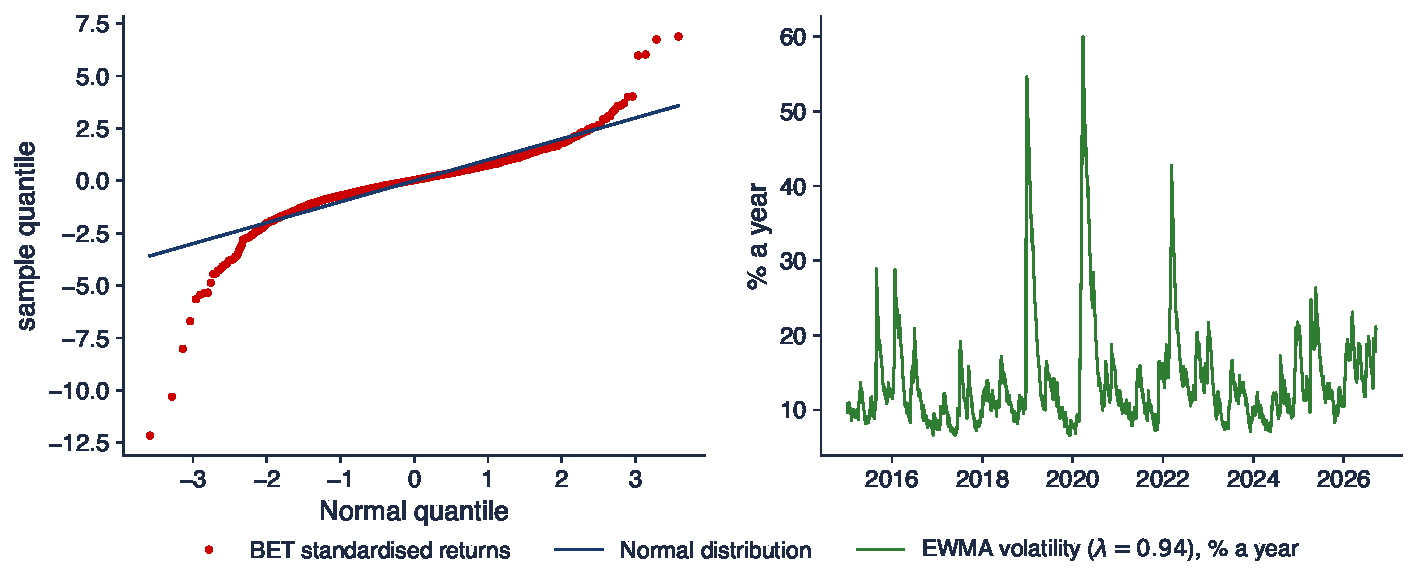
\includegraphics[width=0.96\textwidth,height=0.32\textheight,keepaspectratio]{ch16_sem_b1.pdf}
\end{center}
\vspace{-2mm}
\begin{center}
\scriptsize
\begin{tabular}{llll}
\toprule
\textbf{Performanță} & & \textbf{Distribuție, dependență} & \\
\midrule
media, \% pe an & $13{,}2$ & asimetrie; exces de boltire & $-1{,}41$; $17{,}8$ \\
volatilitate, \% pe an & $15{,}5$ & JB; Hill $\hat\alpha$ (SE) & 39\,794; $2{,}19$ ($0{,}26$) \\
Sharpe (SE) & $0{,}93$ ($0{,}35$) & $Q(10)$: $r_t$; $r_t^2$ & $54{,}7$; $701$ \\
MDD & $-31{,}1\%$ & GARCH-$t$: $\alpha + \beta$; $h_{1/2}$ & $0{,}925$; $8{,}8$ \\
VaR 1\%: HS; Normal & $2{,}72$; $2{,}23$ & ES 2,5\%: HS; Normal & $3{,}21$; $2{,}24$ \\
\bottomrule
\end{tabular}
\end{center}
\begin{itemize}
    \item $n = 2\,925$, 6 ianuarie 2015 -- 18 septembrie 2026; valoarea critică $\chi^2_{0,95}(10) = 18{,}31$; vîrful volatilității EWMA 60{,}0\% la 25 martie 2020
    \item Interpretare: (1) cozi groase: VaR 1\% Normal este prea mic cu 18\%; (2) randamentele sînt slab autocorelate, pătratele lor puternic: volatility clustering; (3) raportul Sharpe se află la mai puțin de trei erori standard de zero
\end{itemize}\sfmquantlet{Ch_16}{SFM_ch16_seminar}
\end{frame}

\begin{frame}{B2: backtesting VaR 1\% pentru S\&P 500 și Bitcoin [Propus]}
\itemsize{\footnotesize}
\begin{itemize}
\item \textbf{Întrebarea}: este mai bună o metodă cu cozi groase decît o metodă Normală cu volatilitate rapidă? Model: B1 și Seminarul 10, B3.
\item \textbf{Date}: S\&P 500 și Bitcoin, toate datele; prognoze pentru fiecare zi de la 1 ianuarie 2017
\item \textbf{Cerințe}
\begin{enumerate}
    \item Calculați VaR 1\% pe o zi prin simulare istorică pe ultimele 500 de randamente.
    \item Calculați VaR 1\% pe o zi EWMA-Normal, cu $\lambda = 0{,}94$.
    \item Numărați depășirile fiecărei metode și aplicați testul Kupiec.
    \item Determinați cel mai mare număr de depășiri din orice 250 de zile consecutive.
    \item Interpretare: ce metodă ar accepta o autoritate de supraveghere pentru fiecare serie?
\end{enumerate}
\item \textbf{Raportați}: un tabel și două fraze
\item Notebook: secțiunea B2
\end{itemize}
\end{frame}

\ifsolutions
\begin{frame}{B2: rezolvare [Propus]}
\itemsize{\footnotesize}
\begin{center}
\scriptsize
\begin{tabular}{l|rrrr|rrrr}
\toprule
& \multicolumn{4}{c|}{HS (500 de zile)} & \multicolumn{4}{c}{EWMA-Normal} \\ & dep. & $LR_{uc}$ & $p$ & max 250 & dep. & $LR_{uc}$ & $p$ & max 250 \\
\midrule
S\&P 500 & 29 (1{,}19\%) & ${0{,}83}$ & 0{,}363 & 10 & 57 (2{,}34\%) & ${31{,}97}$ & $<$\,0{,}001 & 13 \\
Bitcoin & 33 (0{,}93\%) & ${0{,}18}$ & 0{,}672 & 6 & 77 (2{,}17\%) & ${36{,}78}$ & $<$\,0{,}001 & 10 \\
\bottomrule
\end{tabular}
\end{center}
\begin{itemize}
    \item Depășiri așteptate: 24{,}4 (S\&P 500, 2\,440 de zile) și 35{,}5 (Bitcoin, 3\,548 de zile)
    \item EWMA-Normal are de peste două ori rata-țintă pe ambele serii: cuantila Normală este prea mică pentru cozi groase
    \item HS trece testul Kupiec, dar pe S\&P 500 are pînă la 10 depășiri în 250 de zile (zona roșie): reacționează lent
    \item Interpretare: niciuna nu este acceptabilă singură pentru S\&P 500; este nevoie de un model cu filtru de volatilitate și cozi groase (GARCH-$t$, FHS, \sfmchlink{https://danpele.github.io/SFM/RO/Cursuri/capitol10_var_es_backtesting.pdf}{Capitolul 10})
\end{itemize}\sfmquantlet{Ch_16}{SFM_ch16_seminar}
\end{frame}
\fi

\begin{frame}{B3: eficiență și memorie în două ferestre [Propus]}
\itemsize{\footnotesize}
\begin{itemize}
\item \textbf{Întrebarea}: au devenit BET și S\&P 500 mai eficiente după 2015? Model: A3; Seminarul 7, B1 și Seminarul 11, B1.
\item \textbf{Date}: BET și S\&P 500, două ferestre: 2000--2014 și 2015--2026
\item \textbf{Cerințe}
\begin{enumerate}
    \item Calculați VR(5) și $Z^*(5)$ robust în fiecare fereastră.
    \item Calculați exponentul Hurst (R/S) pentru $r_t$ și pentru $|r_t|$ în fiecare fereastră.
    \item Interpretare: a devenit BET mai eficient după 2015?
\end{enumerate}
\item \textbf{Raportați}: un tabel cu șaisprezece valori și două fraze
\item Notebook: secțiunea B3
\end{itemize}
\end{frame}

\ifsolutions
\begin{frame}{B3: rezolvare [Propus]}
\itemsize{\footnotesize}
\begin{center}
\scriptsize
\begin{tabular}{lrrrrrr}
\toprule
& $n$ & VR(5) & $Z^*(5)$ & $p$ & $H$ pentru $r_t$ & $H$ pentru $|r_t|$ \\
\midrule
BET, 2000--2014 & 3\,744 & ${1{,}175}$ & ${2{,}50}$ & 0{,}012 & ${0{,}59}$ & ${0{,}79}$ \\
BET, 2015--2026 & 2\,925 & ${1{,}172}$ & ${1{,}93}$ & 0{,}054 & ${0{,}59}$ & ${0{,}75}$ \\
S\&P 500, 2000--2014 & 3\,770 & ${0{,}822}$ & ${-2{,}63}$ & 0{,}009 & ${0{,}52}$ & ${0{,}84}$ \\
S\&P 500, 2015--2026 & 2\,943 & ${0{,}840}$ & ${-1{,}34}$ & 0{,}181 & ${0{,}53}$ & ${0{,}84}$ \\
\bottomrule
\end{tabular}
\end{center}
\begin{itemize}
    \item BET: VR(5) peste 1 în ambele ferestre (momentum); respins la 5\% înainte de 2015, la limită după
    \item S\&P 500: VR(5) sub 1 (revenire la medie), respins înainte de 2015, nu și după
    \item $H$ pentru $|r_t|$ este de circa 0,75--0,84 în fiecare fereastră: memoria se află în volatilitate, nu în randamente
    \item Interpretare: BET este mai aproape de eficiența în formă slabă după 2015, dar un test aflat la limita de 5\% este o dovadă slabă; următorul pas ar fi ferestrele mobile și benzile Monte Carlo
\end{itemize}\sfmquantlet{Ch_16}{SFM_ch16_seminar}
\end{frame}
\fi


%=============================================================================
\section{Partea C: critica unui răspuns AI}
%=============================================================================

\begin{frame}{C2: verificați un răspuns AI [Propus]}
\itemsize{\scriptsize}
\begin{itemize}
    \item Un student a cerut unui asistent AI să rezume cursul pentru examen, pe datele cursului. Răspunsul:
    \item \aiprompt{(a) VaR 99\% al BET din 2015 este -2{,}72\%.}
    \item \aiprompt{(b) Randamentele BET sînt apropiate de distribuția Normală: asimetria este doar -1{,}41.}
    \item \aiprompt{(c) Bitcoin are o abatere standard zilnică de 3{,}49\%, deci volatilitatea anuală este 55{,}4\%.}
    \item \aiprompt{(d) Pentru S\&P 500, alpha + beta = 0{,}993, deci un șoc de volatilitate se înjumătățește în 1/(1 - 0{,}993) = 139 de zile.}
    \item \aiprompt{(e) Exponentul Hurst pentru |r| este 0{,}84 la S\&P 500, deci randamentele sînt previzibile, iar piața este ineficientă.}
    \item \aiprompt{(f) Pentru randamente Normale, ES 2,5\% și VaR 1\% sînt practic același număr.}
    \item Cerințe
    \begin{itemize}
        \item 1. Pentru fiecare afirmație, precizați dacă este corectă; dacă nu este, formulați afirmația corectă și dați valoarea corectă din notebook (secțiunea C2).
        \item 2. Raportați: o listă de șase verdicte, fiecare cu un rînd de justificare.
    \end{itemize}
\end{itemize}
\end{frame}

\ifsolutions
\begin{frame}{C2: rezolvare [Propus]}
\itemsize{\footnotesize}
\begin{itemize}
    \item (a) Greșit de două ori: nivelul este probabilitatea cozii, VaR 1\%, iar VaR este o pierdere pozitivă: VaR 1\% $= 2{,}72\%$
    \item (b) Greșit: $S = -1{,}41$ este departe de 0 pentru date zilnice, excesul de boltire este $17{,}8$, iar JB $=$ 39\,794
    \item (c) Greșit: Bitcoin se tranzacționează 365 de zile pe an: $\sqrt{365} \times 3{,}49 = 66{,}6\%$
    \item (d) Greșit: timpul de înjumătățire este $\ln 0{,}5/\ln 0{,}993 = 96$ zile; $1/(1 - \alpha - \beta)$ nu este un timp de înjumătățire
    \item (e) Greșit: memoria lui $|r_t|$ este memoria volatilității; pentru $r_t$, $H = 0{,}53$, iar testul VR robust dă $Z^* = -1{,}34$ (nu se respinge)
    \item (f) Corect: $\varphi(1{,}96)/0{,}025 = 2{,}338$, față de $2{,}326$, un raport de 1{,}005
\end{itemize}\sfmquantlet{Ch_16}{SFM_ch16_seminar}
\end{frame}
\fi


%=============================================================================
\section{Încheiere}
%=============================================================================

\begin{frame}{Idei de reținut}
\itemsize{\small}
\begin{itemize}
    \item Orice problemă de examen are trei părți: formula cu cifrele înlocuite, rezultatul cu unitate și semn, interpretarea
    \item Testele: precizați $H_0$, statistica, valoarea critică, decizia; preferați varianta robustă
    \item Riscul: VaR 1\% este o pierdere pozitivă; distribuția Normală îl subestimează pe date reale
    \item Volatilitatea este previzibilă, semnul randamentelor aproape deloc
    \item Un răspuns AI este o ciornă: verificați nivelul și semnul VaR, factorul de anualizare și fiecare formulă
\end{itemize}
\end{frame}

\begin{frame}{După seminar}
\itemsize{\small}
\begin{itemize}
    \item Cursul 16 adună întreaga materie: harta cursului, cîte un slide de recapitulare pentru fiecare capitol, trusa de instrumente, opt probleme de tip examen rezolvate, proiectul
    \item Încercați cerințele [Propus] întîi pe hîrtie, apoi verificați-le în notebook
    \item B3 poate deveni un proiect de echipă: ferestre mobile, benzi Monte Carlo, mai multe piețe emergente
    \item Lectură: \refFHH; exerciții în \refBHL
    \item Seminarul are rol de exercițiu și nu se notează; rezolvările cerințelor [Propus] se discută la seminar
\end{itemize}
\end{frame}


%=============================================================================
\section{Bibliografie}
%=============================================================================

\begin{frame}{Bibliografie}
\itemsize{\tiny}
\begin{itemize}
    \item Adrian, T., Brunnermeier, M.K. (2016). \href{https://doi.org/10.1257/aer.20120555}{CoVaR}. \textit{American Economic Review}, 106(7), 1705--1741.
    \item Bollerslev, T. (1986). \href{https://doi.org/10.1016/0304-4076(86)90063-1}{Generalized autoregressive conditional heteroskedasticity}. \textit{Journal of Econometrics}, 31(3), 307--327.
    \item Borak, S., Härdle, W.K., López-Cabrera, B. (2013). \href{https://doi.org/10.1007/978-3-642-33929-5}{\textit{Statistics of Financial Markets: Exercises and Solutions}}, 2nd ed. Springer.
    \item Franke, J., Härdle, W.K., Hafner, C.M. (2019). \href{https://doi.org/10.1007/978-3-030-13751-9}{\textit{Statistics of Financial Markets: An Introduction}}, 5th ed. Springer.
    \item Hill, B.M. (1975). \href{https://doi.org/10.1214/aos/1176343247}{A simple general approach to inference about the tail of a distribution}. \textit{Annals of Statistics}, 3(5), 1163--1174.
    \item Hurst, H.E. (1951). \href{https://doi.org/10.1061/TACEAT.0006518}{Long-term storage capacity of reservoirs}. \textit{Transactions of the American Society of Civil Engineers}, 116(1), 770--799.
    \item Jarque, C.M., Bera, A.K. (1980). \href{https://doi.org/10.1016/0165-1765(80)90024-5}{Efficient tests for normality, homoscedasticity and serial independence of regression residuals}. \textit{Economics Letters}, 6(3), 255--259.
    \item Kupiec, P.H. (1995). \href{https://doi.org/10.3905/jod.1995.407942}{Techniques for verifying the accuracy of risk measurement models}. \textit{Journal of Derivatives}, 3(2), 73--84.
    \item Lo, A.W., MacKinlay, A.C. (1988). \href{https://doi.org/10.1093/rfs/1.1.41}{Stock market prices do not follow random walks: evidence from a simple specification test}. \textit{Review of Financial Studies}, 1(1), 41--66.
\end{itemize}
\end{frame}

\end{document}
